% !TeX root = ../../金融经济学_王江_讲义及习题.tex
% 知识点：references/金融经济学/金融经济学-王江_261013.pdf，印刷页 67–81
% 习题：references/金融经济学/史上最全最完整的金融经济学答案(王江版).pdf，页 20–25（印刷页 19–24）

\zhchapter{期权：一个套利定价的例子}

\ifdefined\WJHandoutKnowledge

第 4 章给出无套利与资产定价基本定理的一般形式。本章把它们用到\textbf{期权}上：先只靠无套利得到价格的上下界与平价关系，再在完全市场（尤其是二叉树）中得到精确价格；最后说明期权本身也可以把市场完全化。

\begin{tcolorbox}[knowledge,title=5.1 期权]
记标的证券（下文统称股票，也可以是任意证券）在 1 期的支付为 $\tilde{X}$，0 期价格为 $S$。

\begin{tcolorbox}[knowledge]
\textbf{定义 5.1}\quad \textbf{欧式看涨期权}（European call）赋予买方在到期日、以执行价格 $K$ 从期权出售者处买入 1 单位标的证券的权利。\textbf{欧式看跌期权}（European put）则是以执行价格 $K$ 卖出 1 单位标的证券的权利。

在本书的两期框架里只有一个到期日，就是 1 期。$K$ 称为\textbf{执行价格}（exercise price）。因为是权利而不是义务，只有支付为正时才会执行。记欧式看涨、看跌在 1 期的支付为 $\tilde{c}$、$\tilde{p}$，则
\[
    \tilde{c}=[\tilde{X}-K]_{+},\qquad \tilde{p}=[K-\tilde{X}]_{+},
    \tag{5.1}
\]
其中 $[x]_{+}=\max\{0,x\}$。
\end{tcolorbox}

\begin{tcolorbox}[knowledge]
\textbf{定义 5.2}\quad 执行价格为 $K$、到期日为 $t$ 的\textbf{美式看涨（看跌）期权}赋予买方在到期日及此前任一日期，以价格 $K$ 买入（卖出）1 单位标的证券的权利。
\end{tcolorbox}

$S-K$ 称为看涨期权的\textbf{内在价值}（intrinsic value），看跌期权的内在价值是 $K-S$。内在价值大于、等于、小于 $0$ 时，分别称为\textbf{实值}（in the money）、\textbf{平值}（at the money）、\textbf{虚值}（out of the money）。

期权是买方与出售者（\textbf{期权立权人}，option writer）之间的零和合约：买方得到的正支付恰为出售者的付出，净供给恒为 $0$。支付又完全由标的证券的价格决定。满足这两条的证券称为\textbf{衍生证券}（derivative security）。

记 $c(S,K)$、$p(S,K)$ 为欧式看涨、看跌的 0 期价格，$C(S,K)$、$P(S,K)$ 为相应的美式价格。定价分两步：无套利给出基本性质与上下界；完全市场给出精确公式。
\end{tcolorbox}

\begin{tcolorbox}[knowledge,title=5.2 期权价格的性质和界]
欧式期权的支付只在到期日发生，价格由支付决定。影响价格的因素主要有：标的证券的价格与支付、合同条款（执行价格；本书只有一个到期日）、以及决定货币时间价值的利率。

\begin{tcolorbox}[knowledge]
\textbf{定理 5.1}\quad $c(S,K)$ 与 $p(S,K)$ 非负。

支付非负，再由无套利即得。

\textbf{定理 5.2}\quad $c(S,K)$ 对 $K$ 非增，$p(S,K)$ 对 $K$ 非减。

对 $K_1>K_2$，$[\tilde{X}-K_1]_{+}\le[\tilde{X}-K_2]_{+}$，无套利（定价算子单调）给出 $c(S,K_1)\le c(S,K_2)$。看跌类似。

\textbf{定理 5.3}\quad $c(S,K)$ 与 $p(S,K)$ 是 $K$ 的凸函数。

$[\,\cdot\,]_{+}$ 对 $K$ 凸：对 $\alpha\in(0,1)$，
\[
    [\tilde{X}-(\alpha K_1+(1-\alpha)K_2)]_{+}
    \le\alpha[\tilde{X}-K_1]_{+}+(1-\alpha)[\tilde{X}-K_2]_{+}.
\]
定价算子线性且单调，故 $c(S,K)$ 对 $K$ 凸。$[K-\tilde{X}]_{+}$ 同样。

\textbf{定理 5.4}\quad 设 $\theta\ge 0$ 为 $N$ 只证券的组合，价格向量 $S=\begin{bmatrix}S_1\\\vdots\\S_N\end{bmatrix}\gg 0$，执行价格向量 $K=\begin{bmatrix}K_1\\\vdots\\K_N\end{bmatrix}\gg 0$。则
\[
    c(S^{\mathsf T}\theta,\,K^{\mathsf T}\theta)\le\sum_{i=1}^{N}\theta_i\,c(S_i,K_i),
    \qquad
    p(S^{\mathsf T}\theta,\,K^{\mathsf T}\theta)\le\sum_{i=1}^{N}\theta_i\,p(S_i,K_i).
\]
以组合为标的的期权，不比“各证券期权按同样权重组成的组合”更贵。证明来自支付的凸性：
\[
    [(\tilde{X}-K)^{\mathsf T}\theta]_{+}
    \le\sum_{i=1}^{N}\theta_i[\tilde{X}_i-K_i]_{+}.
\]

\textbf{定理 5.5}\quad $S\ge c(S,K)$。

$\tilde{X}\ge[\tilde{X}-K]_{+}$，无套利即得。

\textbf{定理 5.6}\quad 若存在收益率为 $r_F$ 的无风险证券，则
\[
    c(S,K)\ge\Bigl[S-\frac{K}{1+r_F}\Bigr]_{+}.
\]
买入 1 股、卖出面值 $K$（现值为 $K/(1+r_F)$）的无风险证券，现值为 $S-K/(1+r_F)$，1 期支付为 $\tilde{X}-K$。而 $[\tilde{X}-K]_{+}\ge\tilde{X}-K$，故 $c(S,K)\ge S-K/(1+r_F)$。再与 $c\ge 0$ 合并即得。
\end{tcolorbox}

欧式看涨的上下界因此是
\[
    \Bigl[S-\frac{K}{1+r_F}\Bigr]_{+}\le c(S,K)\le S.
    \tag{5.2}
\]

\begin{tcolorbox}[knowledge]
\textbf{定理 5.7（看涨—看跌平价）}\quad 若存在收益率为 $r_F$ 的无风险证券，则
\[
    c(S,K)+\frac{K}{1+r_F}=p(S,K)+S.
    \tag{5.3}
\]
\end{tcolorbox}

比较两个组合：（1）1 份执行价为 $K$ 的看涨，加上面值为 $K$ 的无风险证券（现值为 $K/(1+r_F)$）；（2）1 份执行价为 $K$ 的看跌，加上 1 股股票。
\[
\begin{array}{c|cc}
 & \tilde{X}\le K & \tilde{X}>K \\ \hline
\text{组合 1} & [\tilde{X}-K]_{+}+K=K & [\tilde{X}-K]_{+}+K=\tilde{X} \\
\text{组合 2} & [K-\tilde{X}]_{+}+\tilde{X}=K & [K-\tilde{X}]_{+}+\tilde{X}=\tilde{X}
\end{array}
\]
1 期支付相同，0 期成本必相同，即 (5.3)。看跌的界可由平价从看涨的界推出。
\end{tcolorbox}

\begin{tcolorbox}[knowledge,title=5.3 美式期权以及提前执行]
\textbf{提前执行}（early exercise）是权利不是义务。持有至到期时，美式期权与相应欧式期权支付相同；既然可以等到更优时再执行，美式价格不会低于欧式价格：
\[
    C(S,K)\ge c(S,K),\qquad P(S,K)\ge p(S,K).
    \tag{5.4}
\]
若提前执行以正概率发生，则不等式严格。是否提前执行，与标的在到期前是否支付\textbf{股利}有关。此前默认证券只在 1 期有支付；0 期的支付就是股利。

\begin{tcolorbox}[example]
\begin{question}
\textbf{例 5.1}\quad 0 期股价为 $100$ 的股票支付股利 $100$（如同清算：资产变现 $100$ 并全部作为股利付出）。除息后股价降为 $0$。以此股票为标的、执行价格为 $80$ 的欧式看涨与相应美式看涨，价格分别是多少？提前执行是否最优？
\end{question}
\begin{solution}
1 期股价为 $0$，欧式看涨支付为 $0$，故其价格为 $0$。美式看涨可以在股利发放前执行：支付 $80$ 买入股票，立刻得到股利 $100$，净得 $20$。提前执行严格优于持有至到期，美式看涨价值为 $20$。
\end{solution}
\end{tcolorbox}

因此，分析提前执行时必须把股利考虑进去。先看无股利，再看有股利。

\tcbline

\textbf{A.\ 无股利时的提前执行}

无股利时，美式看涨\textbf{不会}提前执行。立即执行只得到 $S-K$，而
\[
    S-K\le S-\frac{K}{1+r_F}
    \le\Bigl[S-\frac{K}{1+r_F}\Bigr]_{+}
    \le c(S,K)\le C(S,K).
\]
提前执行的所得不超过把同一期权当作欧式期权卖掉的价值；且当 $r_F>0$ 时，在 $S>K$ 的状态下第一个不等式严格，提前执行是次优的。因而
\[
    C(S,K)=c(S,K).
\]
代价来自两处：一是货币的时间价值——行权策略“到期无论股价如何都执行”得到 $\tilde{X}-K$，现值 $S-K/(1+r_F)$，已优于现在就付出 $K$；二是到期可以不执行，$[\tilde{X}-K]_{+}$ 优于 $\tilde{X}-K$。

无股利的美式看跌则可能提前执行。提前执行放弃的是“支付可以更高时不执行”的权利，得到的是现在就收到 $K$、而不是以后才收到。由平价，
\[
    P(S,K)
    =\max\Bigl[K-S,\;p(S,K)\Bigr]
    =\max\Bigl[K-S,\;\frac{K}{1+r_F}-S+c(S,K)\Bigr].
\]
当 $K-S>K/(1+r_F)-S+c(S,K)$，即
\[
    \frac{r_F}{1+r_F}K>c(S,K)
\]
时，提前执行最优。看跌深度实值（$K\gg S$，从而看涨几乎无价值）时，这个不等式成立。

\tcbline

\textbf{B.\ 有股利时的提前执行}

设股票在 $0$ 期还支付股利 $D$，记 $S$ 为\textbf{除息价}。美式看涨在 $0$ 期可以：（1）支付 $K$ 执行并拿到股利，得到 $S+D-K$；或（2）持有至 1 期。最优策略下
\[
    C(S,D,K)=\max\bigl[S+D-K,\;c(S,K)\bigr].
\]
看跌相应为
\[
    P(S,D,K)=\max\bigl[K-S-D,\;p(S,K)\bigr].
\]
由 (5.4)，$C(S,D,K)\ge c(S,K)$、$P(S,D,K)\ge p(S,K)$。因此对美式期权，\textcolor{red}{\textbf{股利促使持有者提前执行看涨、推迟执行看跌}}。

有股利时平价也要改。比较：（1）1 份执行价为 $K$ 的看涨，加上现值为 $K/(1+r_F)+D$ 的无风险证券；（2）1 份执行价为 $K$ 的看跌，加上 1 股股票（$0$ 期得到股利 $D$，并按无风险利率持有至 1 期）。
\[
\begin{array}{c|cc}
 & \tilde{X}\le K & \tilde{X}>K \\ \hline
\text{组合 1} & K+D(1+r_F) & \tilde{X}+D(1+r_F) \\
\text{组合 2} & K+D(1+r_F) & \tilde{X}+D(1+r_F)
\end{array}
\]
支付相同，故
\[
    c(S,K)+\frac{K}{1+r_F}+D=S+p(S,K).
\]
\end{tcolorbox}

\begin{tcolorbox}[knowledge,title=5.4 完全市场中的期权定价]
若证券市场完全，状态价格 $\phi\gg 0$ 唯一。记 $S_\omega$ 为标的在状态 $\omega$ 的支付，则
\[
    c(S,K)
    =\sum_{\omega}\phi_{\omega}[S_{\omega}-K]_{+}
    =\frac{1}{1+r_F}\,\mathrm{E}^{Q}[\tilde{S}-K]_{+},
\]
其中 $Q$ 为风险中性测度。要得到更具体的公式，需要对股价过程再加假设。

\tcbline

\textbf{二叉树。}股价现值为 $S$。下一期以概率 $p$ 变为 $uS$、以概率 $1-p$ 变为 $dS$，设 $u>d$：
\begin{center}
\WJEventTree[left={$S$},stem]{uS\text{，概率 }p, dS\text{，概率 }1-p}
\end{center}
另有无风险证券，1 期支付 $1$，价格 $B=1/(1+r_F)$，利率为 $r_F$。

无套利要求 $d<1+r_F<u$。反证：若 $d\ge 1+r_F$，买入 1 股（支出 $S$），同时卖出 $S(1+r_F)$ 份无风险证券（收入恰为 $S$），0 期净支出为 $0$。1 期上涨时支付 $[u-(1+r_F)]S>0$，下跌时 $[d-(1+r_F)]S\ge 0$，构成套利。故 $d<1+r_F$；同理 $u>1+r_F$。

两个状态、股票与债券的支付线性无关，市场完全，状态价格唯一。$\phi=\begin{bmatrix}\phi_u\\\phi_d\end{bmatrix}\gg 0$ 满足
\[
    S=\phi_u\,uS+\phi_d\,dS,\qquad B=\phi_u+\phi_d,
\]
解得
\[
    \phi_u=\frac{1}{1+r_F}\frac{1+r_F-d}{u-d},
    \qquad
    \phi_d=\frac{1}{1+r_F}\frac{u-(1+r_F)}{u-d}.
\]
欧式看涨价格为
\[
    c=\phi_u[uS-K]_{+}+\phi_d[dS-K]_{+}.
    \tag{5.5}
\]

\tcbline

\textbf{复制。}只有两个状态时，股票和债券使任何其他证券成为冗余证券，其价格等于复制组合的价格。到期支付
\[
    c_u=[uS-K]_{+},\qquad c_d=[dS-K]_{+}.
\]
持有 $\theta_S$ 股与 $\theta_B$ 份面值 $1$ 的债券，使两个状态下的支付分别等于 $c_u$、$c_d$：
\[
    \theta_S\,uS+\theta_B=c_u,\qquad \theta_S\,dS+\theta_B=c_d.
\]
解为
\[
    \theta_S=\frac{c_u-c_d}{(u-d)S},
    \qquad
    \theta_B=\frac{uc_d-dc_u}{u-d}.
\]
$\theta_S$ 称为\textbf{对冲比}（hedge ratio，期权的 $\delta$）。组合在 0 期的价值为 $v=\theta_S S+\theta_B/(1+r_F)$。无套利要求 $c=v$，代回即得 (5.5)。

\tcbline

\textbf{风险中性概率。}定义等价鞅测度
\[
    q=\frac{\phi_u}{\phi_u+\phi_d}=\frac{1+r_F-d}{u-d},
    \qquad
    1-q=\frac{\phi_d}{\phi_u+\phi_d}=\frac{u-(1+r_F)}{u-d}.
\]
则
\[
    c=\frac{1}{1+r_F}\bigl[qc_u+(1-q)c_d\bigr]
    =\frac{\mathrm{E}^{Q}[c_1]}{1+r_F}.
\]
记 $\hat{c}\equiv c/B$、$\hat{S}\equiv S/B$（用无风险债券价格把价格规范化）。在 $Q$ 下 $\hat{c}$ 与 $\hat{S}$ 是鞅：$\hat{c}_t=\mathrm{E}^{Q}[\hat{c}_{t+1}]$，$\hat{S}_t=\mathrm{E}^{Q}[\hat{S}_{t+1}]$。这就是\textbf{二叉树期权定价模型}（binomial model）：完全市场里，期权价格由股票和债券的价格经无套利唯一决定，不需要真实概率 $p$。
\end{tcolorbox}

\begin{tcolorbox}[knowledge,title=5.5 期权与市场完全化]
完全市场中期权是冗余证券，价格由原生证券复制。若期权不是冗余的，引入期权可以扩大可生成的支付，甚至把市场完全化。

\tcbline

\textbf{A.\ 蝴蝶头寸}\quad 同一标的、同一到期日、执行价格不同的欧式看涨可以拼出特定支付。\textbf{蝴蝶头寸}（butterfly）为：买入 1 份执行价 $K-\delta$ 的看涨，卖出 2 份执行价 $K$ 的看涨，买入 1 份执行价 $K+\delta$ 的看涨。1 期支付为
\[
    [\tilde{S}-(K-\delta)]_{+}-2[\tilde{S}-K]_{+}+[\tilde{S}-(K+\delta)]_{+}
    =
    \begin{cases}
        0, & \tilde{S}\le K-\delta,\\
        \tilde{S}-(K-\delta), & K-\delta<\tilde{S}\le K,\\
        -\tilde{S}+(K+\delta), & K<\tilde{S}<K+\delta,\\
        0, & \tilde{S}\ge K+\delta.
    \end{cases}
\]
只有 $\tilde{S}\in(K-\delta,\,K+\delta)$ 时支付非零，形状与状态或有证券类似。

\tcbline

\textbf{B.\ 用期权完全化市场}\quad 若一只证券（或组合）的支付 $\{X_\omega:\omega\in\Omega\}$ 满足 $\omega\neq\omega'$ 时 $X_\omega\neq X_{\omega'}$，称为具有\textbf{状态分离}（state separating）的支付，该证券称为\textbf{状态指数证券}（state-index security）。不妨按支付从小到大编号：$X_1<X_2<\cdots<X_\Omega$。

以它为标的、执行价格为 $X_\omega$ 的欧式看涨，支付为
\[
    [\tilde{X}-X_\omega]_{+}
    =\bigl[0,\ldots,0,\,X_{\omega+1}-X_\omega,\,\ldots,\,X_\Omega-X_\omega\bigr]^{\mathsf T}.
\]
下面 $\Omega$ 只证券的支付矩阵满秩，因而市场完全：1 份状态指数证券，加上执行价格分别为 $X_1,\ldots,X_{\Omega-1}$ 的 $\Omega-1$ 份欧式看涨，
\[
    X=
    \begin{bmatrix}
        X_1 & 0 & 0 & \cdots & 0 \\
        X_2 & X_2-X_1 & 0 & \cdots & 0 \\
        X_3 & X_3-X_1 & X_3-X_2 & \cdots & 0 \\
        \vdots & \vdots & \vdots & \ddots & \vdots \\
        X_\Omega & X_\Omega-X_1 & X_\Omega-X_2 & \cdots & X_\Omega-X_{\Omega-1}
    \end{bmatrix}.
\]

取一个方便计算的例子：状态 $\omega=1,\ldots,\Omega$ 下指数证券支付为 $\delta,2\delta,\ldots,\Omega\delta$。执行价格为 $0,\delta,2\delta,\ldots,(\Omega-1)\delta$ 的看涨（执行价 $0$ 就是标的本身）的支付矩阵为下三角满秩阵
\[
    X=
    \begin{bmatrix}
        \delta & 0 & \cdots & 0 \\
        2\delta & \delta & \cdots & 0 \\
        \vdots & \vdots & \ddots & \vdots \\
        \Omega\delta & (\Omega-1)\delta & \cdots & \delta
    \end{bmatrix}.
\]
执行价为 $n\delta$ 的看涨记为 $X_{\cdot,n}$。蝴蝶头寸“买入执行价 $0$、卖出 2 份执行价 $\delta$、买入执行价 $2\delta$”的支付为
\[
    X_p=(X_{\cdot,0}-X_{\cdot,1})-(X_{\cdot,1}-X_{\cdot,2})
    =[\delta,\delta,\ldots,\delta]^{\mathsf T}-[0,\delta,\ldots,\delta]^{\mathsf T}
    =[\delta,0,\ldots,0]^{\mathsf T},
\]
即 $\delta$ 份状态 $1$ 的或有证券。一般地，执行价 $(i-1)\delta$、$i\delta$、$(i+1)\delta$ 的蝴蝶头寸只在状态 $i$ 支付 $\delta$。因此这组期权可以复制任意状态或有要求权。

记 $\phi_i$ 为状态 $i$ 的状态价格，$K_i=i\delta$。由蝴蝶头寸的价格，
\[
    \phi_i
    =\frac{1}{\delta}\Bigl\{\bigl[c(K_{i-1})-c(K_i)\bigr]-\bigl[c(K_i)-c(K_{i+1})\bigr]\Bigr\}
    =\frac{c(K_{i-1})-2c(K_i)+c(K_{i+1})}{\delta}.
\]
支付为 $\{X_{\omega_i}\}$ 的资产价格为 $S=\sum_i\phi_i X_{\omega_i}$，也即
\[
    S=\sum_i\frac{c(K_{i+1})-2c(K_i)+c(K_{i-1})}{\delta^{2}}\,X_{\omega_i}\,\delta.
\]
状态与 $K_i$ 一一对应，支付可写成 $K$ 的函数 $X(K)$。指数证券连续分布且 $c$ 二阶可导时，取 $\delta=\mathrm{d}K$，二阶差商趋于 $\partial^{2}c/\partial K^{2}$，
\[
    S=\int_{0}^{\infty}\frac{\partial^{2}c(K)}{\partial K^{2}}X(K)\,\mathrm{d}K.
\]
这是 Breeden--Litzenberger 公式。定义风险中性密度
\[
    q(K)
    =\frac{\partial^{2}c(K)/\partial K^{2}}{\displaystyle\int_{0}^{\infty}\partial^{2}c(K)/\partial K^{2}\,\mathrm{d}K}.
\]
无风险债券价格为
\[
    B=\int_{0}^{\infty}\frac{\partial^{2}c(K)}{\partial K^{2}}\,\mathrm{d}K=\frac{1}{1+r_F},
\]
故规范化价格是鞅：
\[
    \frac{S}{B}=\int_{0}^{\infty}q(K)\,X(K)\,\mathrm{d}K.
\]
\end{tcolorbox}

\begin{tcolorbox}[knowledge,title=本章小结]
\begin{enumerate}
    \item 欧式看涨（看跌）是在到期日以执行价格 $K$ 买入（卖出）标的的权利，支付为 $[\tilde{X}-K]_{+}$（$[K-\tilde{X}]_{+}$）。美式期权允许到期日前执行。
    \item 无套利给出欧式看涨的界 $\bigl[S-K/(1+r_F)\bigr]_{+}\le c(S,K)\le S$。
    \item 看涨—看跌平价：$c(S,K)+K/(1+r_F)=p(S,K)+S$。有股利 $D$（$S$ 为除息价）时改为 $c+K/(1+r_F)+D=S+p$。
    \item 美式价格不低于欧式价格。无股利时美式看涨不会提前执行，$C=c$；美式看跌在深度实值时可能提前执行。股利促使提前执行看涨、推迟执行看跌。
    \item 市场完全时，期权由状态价格定价。二叉树中 $d<1+r_F<u$，股票与债券唯一决定状态价格、对冲比和风险中性概率 $q=(1+r_F-d)/(u-d)$，真实概率 $p$ 不进入价格。
    \item 期权不是冗余证券时，状态指数证券上不同执行价的看涨（蝴蝶头寸）可以复制阿罗证券，从而把市场完全化；连续情形下状态价格密度由看涨价格对执行价的二阶导数给出。
\end{enumerate}
\end{tcolorbox}
\fi

% !TeX root = ../../金融经济学_王江_讲义及习题.tex
% 05_期权 课后习题（由章节文件拆分）

\begin{problem}
\problemno{5.1} 1 期有两个可能状态 $a$ 和 $b$，发生概率分别为 $\pi$ 和 $1-\pi$。存在一只收益率为 $r_{F}$ 的无风险证券。还存在一只风险证券，它的现时价格为 $S$，在 1 期支付红利 $\delta S$。它在 1 期的除权价（即红利后的价格）在状态 $a$ 下是 $(1+r_{F}+u)S$、在状态 $b$ 下是 $(1+r_{F}-d)S$。
\begin{enumerate}[label=(\alph*)]
    \item 为使市场中不存在套利机会，$\pi$，$r_{F}$，$u$，$d$ 和 $\delta$ 应该满足什么条件？
    \item 1 期到期、执行价为 $K$ 的欧式买权的 0 期价格是多少？
    \item 美式买权的价格是多少？比较它与相应的欧式买权价格。什么时候提前执行是最优的？
    \item 将买权换成卖权，回答 (b) 和 (c)。
\end{enumerate}
\end{problem}
\begin{solution}
\begin{enumerate}[label=(\alph*)]
    \item $u+\delta>1+r_{F}>d+\delta$；
    \item 令状态价格向量为 $\phi=\begin{bmatrix}\phi_{a} \\ \phi_{b}\end{bmatrix}$，那么有
    \[
        \begin{aligned}
            \phi_{a}+\phi_{b}&=\frac{1}{1+r_{F}}\\
            (u+\delta)S\phi_{a}+(d+\delta)S\phi_{b}&=S
        \end{aligned}
    \]
    求解方程组可得状态价格为
    \[
        \begin{aligned}
            \phi_{a}&=\frac{1}{1+r_{F}}\frac{(1+r_{F})-(d+\delta)}{u-d}\\
            \phi_{b}&=\frac{1}{1+r_{F}}\frac{(u+\delta)-(1+r_{F})}{u-d}
        \end{aligned}
    \]
    因而期权的价格为
    \[
        c=\phi_{a}[uS-K]_{+}+\phi_{b}[dS-K]_{+}=
        \begin{cases}
            0 & uS<K\\
            \phi_{a}(uS-K) & dS\le K\le uS\\
            \phi_{a}(uS-K)+\phi_{b}(dS-K) & K<dS
        \end{cases}
    \]
    \item 对于美式期权来说，如果在 0 期执行，那么获得的收益是 $[S-K]_{+}$，如果在 1 期执行，那么收益和欧式期权一样，因而 $C=\max\{[S-K]_{+},c\}$。当且仅当 $[S-K]_{+}>c$ 时提前执行是最优的。当 $\delta$ 很大时，股价 $S$ 中含有股利的成份越多，因而越有可能提前执行。
    \item 对于欧式看跌期权，价格为
    \[
        p=\phi_{a}[K-uS]_{+}+\phi_{b}[K-dS]_{+}=
        \begin{cases}
            0 & K<dS\\
            \phi_{b}(K-dS) & dS\le K\le uS\\
            \phi_{a}(K-uS)+\phi_{b}(K-dS) & K>uS
        \end{cases}
    \]
    而对于美式看跌期权，$P=\max\{[K-S]_{+},p\}$。当 $\delta$ 越大时，股价 $S$ 中含有股利的成份越多，因而越有可能不提前执行。
\end{enumerate}
\end{solution}

\begin{problem}
\problemno{5.2} 在 1 期有三个可能状态：$\{\omega_{1},\omega_{2},\omega_{3}\}$，在经济中有三只交易证券，它们的支付向量如下：
\[
    X_{a}=\begin{bmatrix}1\\1\\0\end{bmatrix},\quad
    X_{b}=\begin{bmatrix}0\\1\\1\end{bmatrix},\quad
    X_{c}=\begin{bmatrix}1/2\\1\\1/2\end{bmatrix}.
\]
这些证券的 0 期均衡价格是 $S_{a}=S_{b}=S_{c}=1$。令 $\phi=\begin{bmatrix}\phi_{1} \\ \phi_{2} \\ \phi_{3}\end{bmatrix}$ 为状态价格向量。[这与前一章练习 4.5 定义的经济一样。]考虑一份标的资产证券为 $a$、执行价格为 $1/2$ 的欧式买权。它的支付是什么？你能确定它的价格吗？
\end{problem}
\begin{solution}
它的支付是 $\begin{bmatrix}1/2\\1/2\\0\end{bmatrix}$，因为它的支付恰为证券 $a$ 的一半，因而它的价格也是一半即 $\tfrac12$。
\end{solution}

\begin{problem}
\problemno{5.3} 蝴蝶头寸是看涨期权的组合：（1）买入 1 份执行价格为 $K-\delta$ 的看涨期权，（2）卖出 2 份执行价格为 $K$ 的看涨期权，（3）买入 1 份执行价格为 $K+\delta$ 的看涨期权。因此，蝴蝶头寸可由两个参数 $K$ 和 $\delta$ 刻划。比较两个蝴蝶头寸，$K$ 相同但 $\delta$ 不同。证明 $\delta$ 较高的蝴蝶头寸的价值较高。
\end{problem}
\begin{solution}
假设 $\delta_{1}>\delta_{0}$，比较两只期权的支付。当 1 期价格 $S$ 大于 $K+\delta$ 或者小于 $K-\delta$ 时，两者的支付都为 0；当 $S\in[K-\delta_{1},K-\delta_{0}]$ 时 $X_{1}=S-(K-\delta_{1})>X_{0}=0$；当 $S\in[K-\delta_{0},K]$ 时 $X_{1}=S-(K-\delta_{1})>S-(K-\delta_{0})=X_{0}$；当 $S\in[K,K+\delta_{0}]$ 时 $X_{1}=-S+(K+\delta_{1})>-S+(K+\delta_{0})=X_{0}$；当 $S\in[K+\delta_{0},K+\delta_{1}]$ 时 $X_{1}=-S+(K+\delta_{1})>0=X_{0}$；根据无套利原理，$\delta$ 较高的期权价格较高。
\end{solution}

\begin{problem}
\problemno{5.4} 对于参数为 $K$ 和 $\delta$ 的蝴蝶头寸，给出它的价格的一个上界和下界。
\end{problem}
\begin{solution}
一个上界是 $[S-(K-\delta)]_{+}-[S-(K+\delta)]_{+}$，因为期权的支付是非负的，因而 0 是它的一个下界。
\end{solution}

\begin{problem}
\problemno{5.5} 股票价格具有如下形式的二叉树结构：
\begin{center}
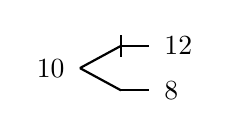
\begin{tikzpicture}[x=1.35em,y=1.15em,baseline=(current bounding box.center)]
    \node[anchor=east] at (-0.15,0) {$10$};
    \draw[thick] (0,0) -- (1.1,0.7);
    \draw[thick] (0,0) -- (1.1,-0.7);
    \draw[thick] (1.1,0.35) -- (1.1,1.05);
    \draw[thick] (1.1,0.7) -- (1.85,0.7);
    \draw[thick] (1.1,-0.7) -- (1.85,-0.7);
    \node[anchor=west] at (2.0,0.7) {$12$};
    \node[anchor=west] at (2.0,-0.7) {$8$};
\end{tikzpicture}
\end{center}
两个可能结果的发生概率相等，无风险利率是 $10\%$。
\begin{enumerate}[label=(\alph*)]
    \item 为一个以此股票为标的资产、执行价格为 9 的看跌期权定价。
    \item 假设你得到一个新的利好信息：股票价格上升到 12 的概率大于 $1/2$，而股票价格仍然是 10。你愿意支付的看跌期权的价格是上涨还是下跌？解释原因。
\end{enumerate}
\end{problem}
\begin{solution}
\begin{enumerate}[label=(\alph*)]
    \item 由第 1 题中公式可以得到状态价格为 $\phi=[\tfrac{15}{22},\tfrac{5}{22}]$，因而看跌期权的价格为 $\dfrac{5}{22}\times[9-8]=\dfrac{5}{22}$；
    \item 由于股价不变，状态价格也不会变化，因而看跌期权的价格是不变的。
\end{enumerate}
\end{solution}

\begin{problem}
\problemno{5.6} 二叉树模型可以拓展到多于两个时期的情形。考虑拓展到三个时期 0，1，2 的情况。股票价格服从如下的二叉树过程：
\begin{center}
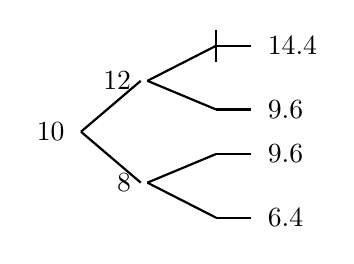
\begin{tikzpicture}[x=1.6em,y=1.15em,baseline=(current bounding box.center)]
    \node[anchor=east] at (0,0) {$10$};
    \draw[thick] (0.15,0) -- (1.5,1.6);
    \draw[thick] (0.15,0) -- (1.5,-1.6);
    \node[anchor=east] at (1.5,1.6) {$12$};
    \node[anchor=east] at (1.5,-1.6) {$8$};
    \draw[thick] (1.65,1.6) -- (3.2,2.7);
    \draw[thick] (1.65,1.6) -- (3.2,0.7);
    \draw[thick] (1.65,-1.6) -- (3.2,-0.7);
    \draw[thick] (1.65,-1.6) -- (3.2,-2.7);
    \draw[thick] (3.2,2.2) -- (3.2,3.2);
    \draw[thick] (3.2,2.7) -- (4.0,2.7);
    \draw[thick] (3.2,0.7) -- (4.0,0.7);
    \draw[thick] (3.2,-0.7) -- (4.0,-0.7);
    \draw[thick] (3.2,-2.7) -- (4.0,-2.7);
    \node[anchor=west] at (4.15,2.7) {$14.4$};
    \node[anchor=west] at (4.15,0.7) {$9.6$};
    \node[anchor=west] at (4.15,-0.7) {$9.6$};
    \node[anchor=west] at (4.15,-2.7) {$6.4$};
\end{tikzpicture}
\end{center}
每一期间（即，从 0 期到 1 期或从 1 期到 2 期）的利率都是 $10\%$。考虑一份在 2 期到期、执行价格为 9 的看涨期权。
\begin{enumerate}[label=(\alph*)]
    \item 描述这份看涨期权在 2 期的支付。
    \item 求解看涨期权在 1 期、股票价格分别为 12 或 8 时的价格。
    \item 求解看涨期权在 0 期的价格。
    \item 如果是美式看涨期权，它在 0 期的价格是多少？
\end{enumerate}
\end{problem}
\begin{solution}
\begin{enumerate}[label=(\alph*)]
    \item 支付是
    \[
        \begin{bmatrix}5.4\\0.6\\0.6\\0\end{bmatrix}
    \]
    \item 可以求得每个节点的状态价格都和第 5 题中的一样。当股价为 12 时，期权价格为 $\dfrac{15}{22}\times 5.4+\dfrac{5}{22}\times 0.6=3.82$；当股价为 8 时，期权价格为 $\dfrac{15}{22}\times 0.6=0.41$；
    \item 看涨期权的 0 期价格为 $\dfrac{15}{22}\times 3.82+\dfrac{5}{22}\times 0.41=2.70$；
    \item 因为没有股利，美式看涨期权不会提前执行，价格也是 2.70。
\end{enumerate}
\end{solution}

\begin{problem}
\problemno{5.7*} 在练习 5.6 描述的经济中，考虑一份以股票为标的资产、在 2 期到期、执行价格为 14 的看跌期权。
\begin{enumerate}[label=(\alph*)]
    \item 如果它是欧式期权，求解它的 0 期价格。
    \item 如果它是美式期权，求解它的 0 期价格。
\end{enumerate}
\end{problem}
\begin{solution}
\begin{enumerate}[label=(\alph*)]
    \item 期权的 2 期支付是 $\begin{bmatrix}0\\4.4\\4.4\\7.6\end{bmatrix}$；在 1 期，当股价为 12 时，期权价格为 $\dfrac{5}{22}\times 4.4=1$；当股价为 8 时，期权价格为 $\dfrac{15}{22}\times 4.4+\dfrac{5}{22}\times 7.6=4.73$；因而期权的 0 期价格为 $\dfrac{15}{22}\times 1+\dfrac{5}{22}\times 4.73=1.76$。
    \item 期权的 2 期支付是 $\begin{bmatrix}0\\4.4\\4.4\\7.6\end{bmatrix}$；在 1 期如果不提前执行，当股价为 12 时，期权价格为 $\dfrac{5}{22}\times 4.4=1$；当股价为 8 时，期权价格为 $\dfrac{15}{22}\times 4.4+\dfrac{5}{22}\times 7.6=4.73$；而如果在 1 期提前执行，那么期权的支付分别为 2 和 6，因而参与者会提前执行，期权在 1 期的支付为 $\begin{bmatrix}2 \\ 6\end{bmatrix}$；如果在 0 期不提前执行，期权的价格为 $\dfrac{15}{22}\times 2+\dfrac{5}{22}\times 6=2.73$，而如果在 0 期提前执行，参与者的收益是 4，因此参与者在 0 期就执行期权，期权在 0 期的价格是 4。
\end{enumerate}
\end{solution}

\begin{problem}
\problemno{5.8*} 这里的经济与练习 5.6 描述的经济一样，只是这里的参数更一般性：
\begin{center}
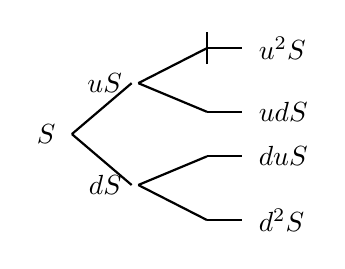
\begin{tikzpicture}[x=1.6em,y=1.15em,baseline=(current bounding box.center)]
    \node[anchor=east] at (0,0) {$S$};
    \draw[thick] (0.15,0) -- (1.5,1.6);
    \draw[thick] (0.15,0) -- (1.5,-1.6);
    \node[anchor=east] at (1.5,1.6) {$uS$};
    \node[anchor=east] at (1.5,-1.6) {$dS$};
    \draw[thick] (1.65,1.6) -- (3.2,2.7);
    \draw[thick] (1.65,1.6) -- (3.2,0.7);
    \draw[thick] (1.65,-1.6) -- (3.2,-0.7);
    \draw[thick] (1.65,-1.6) -- (3.2,-2.7);
    \draw[thick] (3.2,2.2) -- (3.2,3.2);
    \draw[thick] (3.2,2.7) -- (4.0,2.7);
    \draw[thick] (3.2,0.7) -- (4.0,0.7);
    \draw[thick] (3.2,-0.7) -- (4.0,-0.7);
    \draw[thick] (3.2,-2.7) -- (4.0,-2.7);
    \node[anchor=west] at (4.15,2.7) {$u^{2}S$};
    \node[anchor=west] at (4.15,0.7) {$udS$};
    \node[anchor=west] at (4.15,-0.7) {$duS$};
    \node[anchor=west] at (4.15,-2.7) {$d^{2}S$};
\end{tikzpicture}
\end{center}
每一期间的利率都是 $r_{F}$ 且 $0<d<1+r_{F}<u$。
\begin{enumerate}[label=(\alph*)]
    \item 求解在每一时期考虑下一期的两种可能情形（即股价上升或下降）的风险中性概率。
    \item 用 $S$，$u$，$d$ 和 $r_{F}$ 表示欧式看跌期权在 0 期的价格。
    \item 证明在 2 期到期的美式看涨期权的价格比具有相同执行价格、但在 1 期到期的美式看涨期权的价格要高。
\end{enumerate}
\end{problem}
\begin{solution}
\begin{enumerate}[label=(\alph*)]
    \item 状态价格在每期都是一样的，
    \[
        \begin{aligned}
            \phi_{u}&=\frac{1}{1+r_{F}}\frac{(1+r_{F})-d}{u-d}\\
            \phi_{d}&=\frac{1}{1+r_{F}}\frac{u-(1+r_{F})}{u-d}
        \end{aligned}
    \]
    因此，每一个节点处的风险中性概率也是一样的，
    \[
        q_{u}=\frac{(1+r_{F})-d}{u-d},\quad q_{d}=\frac{u-(1+r_{F})}{u-d}
    \]
    \item 欧式看跌期权在 0 期的价格为
    \[
        \begin{aligned}
            &\phi_{u}\bigl(\phi_{u}[K-u^{2}S]_{+}+\phi_{d}[K-udS]_{+}\bigr)+\phi_{d}\bigl(\phi_{u}[K-udS]_{+}+\phi_{d}[K-d^{2}S]_{+}\bigr)\\
            &=\phi_{u}^{2}[K-u^{2}S]_{+}+2\phi_{u}\phi_{d}[K-udS]_{+}+\phi_{d}^{2}[K-d^{2}S]_{+}
        \end{aligned}
    \]
    \item 因为美式期权可以提前执行，在 2 期到期的期权既可以选在 1 期执行也可以选择在 2 期执行，而在 1 期到期的美式看涨期权只会选择在 1 期执行（虽然都可以在 0 期执行，但是在没有股利的情况下，美式看涨期权是不会提前执行的），因而在 2 期到期的期权价格更高。
\end{enumerate}
\end{solution}

\begin{problem}
\problemno{5.9*} 考虑练习 5.8 描述的经济。假设一只证券在 2 期的支付是股票价格从 0 期到 2 期所达到的最大值。（这是一个关于回望期权的例子，它的支付依赖于标的证券的价格路径）。
\begin{enumerate}[label=(\alph*)]
    \item 写出它在 2 期的支付。
    \item 导出它的 0 期价格。
    \item 证明用在 2 期支付一美元的无风险债券的价格正规化以后，这只证券的价格过程在等价鞅测度下是鞅。
\end{enumerate}
\end{problem}
\begin{solution}
这里只考虑 $ud<1$ 的情形，其它情形可以类似考虑。
\begin{enumerate}[label=(\alph*)]
    \item 期权在 2 期的支付是
    \[
        \begin{bmatrix}u^{2}S\\uS\\S\end{bmatrix}
    \]
    \item 0 期价格为 $\phi_{u}^{2}u^{2}S+\phi_{u}\phi_{d}(u+1)S+\phi_{d}^{2}S$；
    \item 在 1 期，当股价为 $uS$ 时，
    \[
        \mathrm{E}^{Q}[\tilde{X}_{2}]=\frac{1}{\phi_{u}+\phi_{d}}(\phi_{u}u^{2}S+\phi_{d}uS)
    \]
    而正规化后的价格为
    \[
        (\phi_{u}u^{2}S+\phi_{d}uS)\Big/\frac{1}{1+r_{F}}=(1+r_{F})(\phi_{u}u^{2}S+\phi_{d}uS)=\frac{1}{\phi_{u}+\phi_{d}}(\phi_{u}u^{2}S+\phi_{d}uS)
    \]
    可以验证其它各节点均如此，因而期权的价格过程为鞅。
\end{enumerate}
\end{solution}

\begin{problem}
\problemno{5.10} 经济在 1 期有 3 个状态。状态一指数证券在三个状态下的支付分别为 1，2，3：
\begin{center}
\WJEventTree[stem]{1,2,3}
\end{center}
并有两只以指数证券为标的资产、执行价格分别为 1 和 2 的看涨期权。用指数证券和上述期权复制如下支付：
\begin{center}
\WJEventTree[stem]{1,1,1}
\qquad
\WJEventTree[stem]{3,2,1}
\qquad
\WJEventTree[stem]{1,0,0}
\end{center}
\end{problem}
\begin{solution}
记状态指数证券的支付向量为 $X_{0}=\begin{bmatrix}1\\2\\3\end{bmatrix}$，执行价格为 1 的指数期权的支付向量为 $X_{1}=\begin{bmatrix}0\\1\\2\end{bmatrix}$，执行价格为 2 的指数期权的支付向量为 $X_{2}=\begin{bmatrix}0\\0\\1\end{bmatrix}$ 那么我们可得：
\[
    X_{0}-X_{1}=\begin{bmatrix}1\\1\\1\end{bmatrix},\quad
    3X_{0}-4X_{1}=\begin{bmatrix}3\\2\\1\end{bmatrix},\quad
    X_{0}+X_{2}-2X_{1}=\begin{bmatrix}1\\0\\0\end{bmatrix}.
\]
\end{solution}


